% generated by tools/make_tikz_figures.py; do not edit
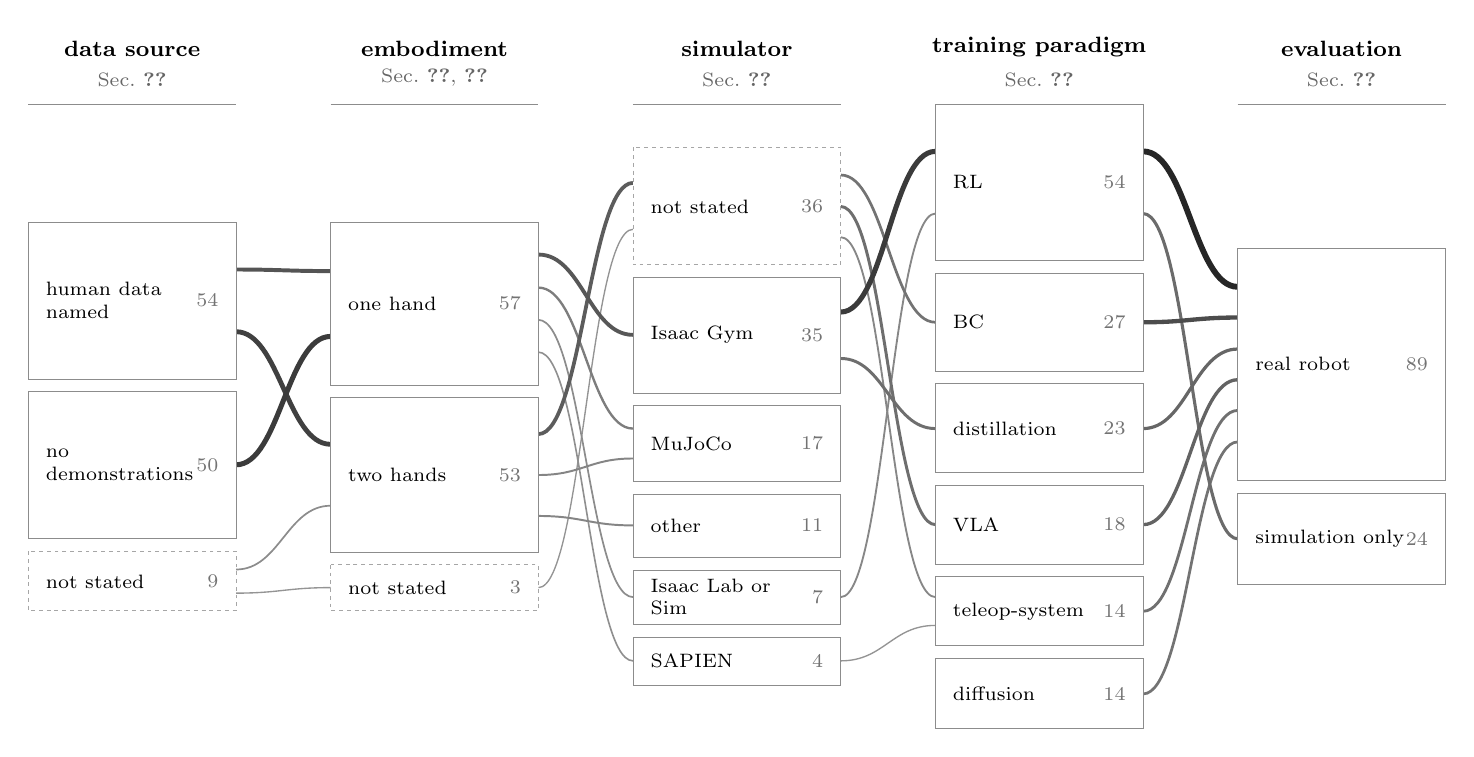
\begin{tikzpicture}[
  font=\scriptsize,
  bar/.style={draw=none,fill=black!62},
  barlight/.style={draw=none,fill=black!22},
  baracc/.style={draw=none,fill=accent},
  box/.style={draw=black!45,line width=0.3pt,inner sep=3pt,align=left},
  ghost/.style={draw=black!35,line width=0.3pt,dash pattern=on 1.4pt off 1.4pt,inner sep=3pt,align=left},
  lnk/.style={draw=black!38,line width=0.28pt},
  lbl/.style={font=\scriptsize},
  num/.style={font=\scriptsize\color{black!55}},
]

\draw[draw=black!42,line width=0.49pt] (2.64,-6.21) .. controls (3.19,-6.21) and (3.29,-6.14) .. (3.84,-6.14);
\draw[draw=black!42,line width=0.49pt] (6.48,-6.14) .. controls (7.03,-6.14) and (7.13,-1.59) .. (7.68,-1.59);
\draw[draw=black!42,line width=0.49pt] (10.32,-7.07) .. controls (10.87,-7.07) and (10.97,-6.62) .. (11.52,-6.62);
\draw[draw=black!44,line width=0.58pt] (6.48,-3.15) .. controls (7.03,-3.15) and (7.13,-7.07) .. (7.68,-7.07);
\draw[draw=black!45,line width=0.62pt] (2.64,-5.91) .. controls (3.19,-5.91) and (3.29,-5.10) .. (3.84,-5.10);
\draw[draw=black!45,line width=0.62pt] (6.48,-2.74) .. controls (7.03,-2.74) and (7.13,-6.26) .. (7.68,-6.26);
\draw[draw=black!47,line width=0.67pt] (10.32,-1.69) .. controls (10.87,-1.69) and (10.97,-6.26) .. (11.52,-6.26);
\draw[draw=black!47,line width=0.67pt] (10.32,-6.26) .. controls (10.87,-6.26) and (10.97,-1.39) .. (11.52,-1.39);
\draw[draw=black!48,line width=0.71pt] (6.48,-4.71) .. controls (7.03,-4.71) and (7.13,-4.50) .. (7.68,-4.50);
\draw[draw=black!48,line width=0.71pt] (6.48,-5.23) .. controls (7.03,-5.23) and (7.13,-5.35) .. (7.68,-5.35);
\draw[draw=black!51,line width=0.85pt] (6.48,-2.33) .. controls (7.03,-2.33) and (7.13,-4.12) .. (7.68,-4.12);
\draw[draw=black!55,line width=0.98pt] (10.32,-0.90) .. controls (10.87,-0.90) and (10.97,-2.77) .. (11.52,-2.77);
\draw[draw=black!55,line width=0.98pt] (14.16,-7.49) .. controls (14.71,-7.49) and (14.81,-4.29) .. (15.36,-4.29);
\draw[draw=black!56,line width=1.03pt] (14.16,-6.44) .. controls (14.71,-6.44) and (14.81,-3.89) .. (15.36,-3.89);
\draw[draw=black!57,line width=1.07pt] (10.32,-1.30) .. controls (10.87,-1.30) and (10.97,-5.34) .. (11.52,-5.34);
\draw[draw=black!57,line width=1.07pt] (10.32,-3.23) .. controls (10.87,-3.23) and (10.97,-4.12) .. (11.52,-4.12);
\draw[draw=black!58,line width=1.12pt] (14.16,-1.39) .. controls (14.71,-1.39) and (14.81,-5.52) .. (15.36,-5.52);
\draw[draw=black!60,line width=1.16pt] (14.16,-4.12) .. controls (14.71,-4.12) and (14.81,-3.11) .. (15.36,-3.11);
\draw[draw=black!61,line width=1.21pt] (14.16,-5.34) .. controls (14.71,-5.34) and (14.81,-3.50) .. (15.36,-3.50);
\draw[draw=black!64,line width=1.34pt] (6.48,-4.19) .. controls (7.03,-4.19) and (7.13,-1.00) .. (7.68,-1.00);
\draw[draw=black!66,line width=1.38pt] (6.48,-1.91) .. controls (7.03,-1.91) and (7.13,-2.93) .. (7.68,-2.93);
\draw[draw=black!67,line width=1.43pt] (2.64,-2.10) .. controls (3.19,-2.10) and (3.29,-2.12) .. (3.84,-2.12);
\draw[draw=black!70,line width=1.56pt] (14.16,-2.77) .. controls (14.71,-2.77) and (14.81,-2.71) .. (15.36,-2.71);
\draw[draw=black!75,line width=1.74pt] (2.64,-2.89) .. controls (3.19,-2.89) and (3.29,-4.32) .. (3.84,-4.32);
\draw[draw=black!77,line width=1.83pt] (2.64,-4.58) .. controls (3.19,-4.58) and (3.29,-2.95) .. (3.84,-2.95);
\draw[draw=black!77,line width=1.83pt] (10.32,-2.64) .. controls (10.87,-2.64) and (10.97,-0.60) .. (11.52,-0.60);
\draw[draw=black!85,line width=2.10pt] (14.16,-0.60) .. controls (14.71,-0.60) and (14.81,-2.32) .. (15.36,-2.32);
\node[font=\footnotesize\bfseries,anchor=south] at (1.32,0.48) {data source};
\node[font=\scriptsize\color{black!60},anchor=south] at (1.32,0.10) {Sec.~\ref{sec:train:human}};
\draw[draw=black!45,line width=0.4pt] (0.00,0.00) -- (2.64,0.00);
\draw[box,fill=white] (0.00,-1.50) rectangle (2.64,-3.49);
\node[lbl,anchor=west,align=left] at (0.10,-2.49) {human data\\named};
\node[num,anchor=east] at (2.54,-2.49) {54};
\draw[box,fill=white] (0.00,-3.65) rectangle (2.64,-5.52);
\node[lbl,anchor=west,align=left] at (0.10,-4.58) {no\\demonstrations};
\node[num,anchor=east] at (2.54,-4.58) {50};
\draw[ghost,fill=white] (0.00,-5.68) rectangle (2.64,-6.43);
\node[lbl,anchor=west,align=left] at (0.10,-6.06) {not stated};
\node[num,anchor=east] at (2.54,-6.06) {9};
\node[font=\footnotesize\bfseries,anchor=south] at (5.16,0.48) {embodiment};
\node[font=\scriptsize\color{black!60},anchor=south] at (5.16,0.10) {Sec.~\ref{sec:hands},~\ref{sec:bimanual}};
\draw[draw=black!45,line width=0.4pt] (3.84,0.00) -- (6.48,0.00);
\draw[box,fill=white] (3.84,-1.50) rectangle (6.48,-3.57);
\node[lbl,anchor=west,align=left] at (3.94,-2.53) {one hand};
\node[num,anchor=east] at (6.38,-2.53) {57};
\draw[box,fill=white] (3.84,-3.73) rectangle (6.48,-5.69);
\node[lbl,anchor=west,align=left] at (3.94,-4.71) {two hands};
\node[num,anchor=east] at (6.38,-4.71) {53};
\draw[ghost,fill=white] (3.84,-5.85) rectangle (6.48,-6.43);
\node[lbl,anchor=west,align=left] at (3.94,-6.14) {not stated};
\node[num,anchor=east] at (6.38,-6.14) {3};
\node[font=\footnotesize\bfseries,anchor=south] at (9.00,0.48) {simulator};
\node[font=\scriptsize\color{black!60},anchor=south] at (9.00,0.10) {Sec.~\ref{sec:simulators}};
\draw[draw=black!45,line width=0.4pt] (7.68,0.00) -- (10.32,0.00);
\draw[ghost,fill=white] (7.68,-0.55) rectangle (10.32,-2.04);
\node[lbl,anchor=west,align=left] at (7.78,-1.30) {not stated};
\node[num,anchor=east] at (10.22,-1.30) {36};
\draw[box,fill=white] (7.68,-2.20) rectangle (10.32,-3.67);
\node[lbl,anchor=west,align=left] at (7.78,-2.93) {Isaac Gym};
\node[num,anchor=east] at (10.22,-2.93) {35};
\draw[box,fill=white] (7.68,-3.83) rectangle (10.32,-4.79);
\node[lbl,anchor=west,align=left] at (7.78,-4.31) {MuJoCo};
\node[num,anchor=east] at (10.22,-4.31) {17};
\draw[box,fill=white] (7.68,-4.95) rectangle (10.32,-5.76);
\node[lbl,anchor=west,align=left] at (7.78,-5.35) {other};
\node[num,anchor=east] at (10.22,-5.35) {11};
\draw[box,fill=white] (7.68,-5.92) rectangle (10.32,-6.61);
\node[lbl,anchor=west,align=left] at (7.78,-6.26) {Isaac Lab or\\Sim};
\node[num,anchor=east] at (10.22,-6.26) {7};
\draw[box,fill=white] (7.68,-6.77) rectangle (10.32,-7.38);
\node[lbl,anchor=west,align=left] at (7.78,-7.07) {SAPIEN};
\node[num,anchor=east] at (10.22,-7.07) {4};
\node[font=\footnotesize\bfseries,anchor=south] at (12.84,0.48) {training paradigm};
\node[font=\scriptsize\color{black!60},anchor=south] at (12.84,0.10) {Sec.~\ref{sec:training}};
\draw[draw=black!45,line width=0.4pt] (11.52,0.00) -- (14.16,0.00);
\draw[box,fill=white] (11.52,-0.00) rectangle (14.16,-1.99);
\node[lbl,anchor=west,align=left] at (11.62,-0.99) {RL};
\node[num,anchor=east] at (14.06,-0.99) {54};
\draw[box,fill=white] (11.52,-2.15) rectangle (14.16,-3.39);
\node[lbl,anchor=west,align=left] at (11.62,-2.77) {BC};
\node[num,anchor=east] at (14.06,-2.77) {27};
\draw[box,fill=white] (11.52,-3.55) rectangle (14.16,-4.68);
\node[lbl,anchor=west,align=left] at (11.62,-4.12) {distillation};
\node[num,anchor=east] at (14.06,-4.12) {23};
\draw[box,fill=white] (11.52,-4.84) rectangle (14.16,-5.84);
\node[lbl,anchor=west,align=left] at (11.62,-5.34) {VLA};
\node[num,anchor=east] at (14.06,-5.34) {18};
\draw[box,fill=white] (11.52,-6.00) rectangle (14.16,-6.88);
\node[lbl,anchor=west,align=left] at (11.62,-6.44) {teleop-system};
\node[num,anchor=east] at (14.06,-6.44) {14};
\draw[box,fill=white] (11.52,-7.04) rectangle (14.16,-7.93);
\node[lbl,anchor=west,align=left] at (11.62,-7.49) {diffusion};
\node[num,anchor=east] at (14.06,-7.49) {14};
\node[font=\footnotesize\bfseries,anchor=south] at (16.68,0.48) {evaluation};
\node[font=\scriptsize\color{black!60},anchor=south] at (16.68,0.10) {Sec.~\ref{sec:evaluation}};
\draw[draw=black!45,line width=0.4pt] (15.36,0.00) -- (18.00,0.00);
\draw[box,fill=white] (15.36,-1.83) rectangle (18.00,-4.78);
\node[lbl,anchor=west,align=left] at (15.46,-3.30) {real robot};
\node[num,anchor=east] at (17.90,-3.30) {89};
\draw[box,fill=white] (15.36,-4.94) rectangle (18.00,-6.10);
\node[lbl,anchor=west,align=left] at (15.46,-5.52) {simulation only};
\node[num,anchor=east] at (17.90,-5.52) {24};
\end{tikzpicture}
